\documentclass[russian,utf8,simple,hpadding=10mm,vpadding=20mm]{eskdtext}
\usepackage[russian]{babel}
\usepackage[T2A]{fontenc}
\usepackage{longtable}
\usepackage{graphicx}
\usepackage{mathtext}
\usepackage[numberright]{eskdplain}
\usepackage[utf8]{inputenc}
\usepackage{listings}
\usepackage{color}
\usepackage{setspace}
\usepackage{dirtree}
\usepackage{multirow}

\definecolor{dkgreen}{rgb}{0,0.6,0}
\definecolor{gray}{rgb}{0.5,0.5,0.5}
\definecolor{mauve}{rgb}{0.58,0,0.82}
\definecolor{light-gray}{gray}{0.25}

\lstdefinestyle{java}{
  language=Java,
  aboveskip=3mm,
  belowskip=3mm,
  showstringspaces=false,
  columns=flexible,
  basicstyle={\footnotesize\ttfamily},
  numberstyle={\tiny},
  numbers=left,
  keywordstyle=\color{blue},
  commentstyle=\color{dkgreen},
  stringstyle=\color{mauve},
  breaklines=true,
  breakatwhitespace=true,
  tabsize=3
}

\lstdefinestyle{xml}{
  language=XML,
  aboveskip=3mm,
  belowskip=3mm,
  showstringspaces=false,
  columns=flexible,
  basicstyle={\footnotesize\ttfamily},
  numberstyle={\tiny},
  numbers=left,
  keywordstyle=\color{blue},
  commentstyle=\color{dkgreen},
  stringstyle=\color{mauve},
  breaklines=true,
  breakatwhitespace=true,
  tabsize=3,
  morekeywords={AnchorPane, children, TreeView, TableView, placeholder, Label, columns, TableColumn, font, Font, Button, import}
}

\ESKDdepartment{Негосударственное образовательное учреждение высшего профессионального образования}
\ESKDcompany{Университет управления «ТИСБИ»}
\renewcommand{\ESKDtitleFontIV}{\LARGE}
\renewcommand{\ESKDtheTitleFieldIV}{КУРСОВАЯ РАБОТА}
\renewcommand{\ESKDtitleFontV}{\Large}
\renewcommand{\ESKDtheTitleFieldV}{По дисциплине: «Объектно-ориентированное программирование»}
\renewcommand{\ESKDtheTitleFieldX}{Казань,~2017г.}
\renewcommand{\ESKDtheTitleFieldVIII}{
\null\hfill
\begin{minipage}{0.5\textwidth}
\normalsize Выполнил 
\\студент гр. ДЗИ 105Н Фомин~А.~В.
\\Руководитель:
\\Козин~А.~Н.
\end{minipage}\\}
\ESKDdate{2017/07/21}
\renewcommand{\thefootnote}{\arabic{footnote}}
\begin{document}
\maketitle
\newpage

\sloppy

\linespread{1,5}
\tableofcontents

\newpage
\parindent=15mm
\doublespacing
\section{Постановка задачи}

Разработать объектную программу для хранения и обработки данных о процессах и используемых ими страницах основной памяти в многозадачных ОС. Каждый процесс имеет уникальный идентификатор и рассматривается как набор страниц. В свою очередь каждая страница имеет уникальный номер и параметр «Состояние».

Разработка включает в себя определение необходимых объектов и описание их в виде классов, программную реализацию методов добавления и удаления процессов и страниц, всестороннее тестирование методов с помощью консольного (при разработке) и оконного (в окончательном варианте) приложения.

Для объединения процессов используется структура данных в виде адресного разомкнутого упорядоченного однонаправленного списка без заголовка. Для объединения страниц внутри процессов  используется очередь на основе обычного массива со сдвигом элементов.

Разработка выполняется с учетом следующих требований:

\begin{itemize}
\item Имена классов, свойств и методов должны носить содержательный смысл и соответствовать информационной задаче
\item Обязательное соблюдение принципа инкапсуляции – использование в классах только закрытых свойств и реализация необходимого набора методов доступа
\item Наличие двух методов для сохранения всей объектной структуры во внешнем файле с обратной загрузкой, при этом стандартные механизмы сериализации разрешается использовать только как дополнение к самостоятельно реализованным методам
\item Тестовое оконное приложение должно обладать удобным пользовательским интерфейсом с контролем вводимых данных и отображением текущего состояния объектной структуры с помощью списковых или табличных компонентов
\item Стандартные контейнеры/коллекции (включая обобщенные классы) разрешается использовать только как дополнение к самостоятельно разработанным классам
\end{itemize}
 
В качестве языка разработки разрешается использовать  Java, С#, C++, Object/Free Pascal и соответствующие инструменты быстрой разработки приложений.

\newpage
\parindent=15mm
\doublespacing
\newcommand{\putimage}[3][1]{
  \begin{figure}[!h]
  \center{\includegraphics[width=#1\linewidth]{#2}}
  \caption{#3}
  \label{ris:#2}
  \end{figure}
}

\section{Описание используемых структур данных с алгоритмами выполнения основных операций}

При реализации задачи мною был реализован класс списка процессов при помощи упорядоченного однонаправленного связанного списка и класс очереди страниц памяти на основе обычного массива со сдвигом элементов.

Класс списка процессов ProcessesList содержит в себе внутренний класс ListItem, который является списковым контейнером и содержит в себе объект класса Process, ссылку на следующий объект контейнера в списке. Помимо базовых геттеров и сеттеров для установки и чтения объектов класса Process и следущего элемента, класс ListItem содержит метод isSmallerThan, необходимый для сравнения с другим объектом класса ListItem. Результатом выполнения этого метода является boolean значение. Если оно принимает значение true, то это означает что текущий объект класса ListItem меньше переданного объекта класса ListItem. Если значение false, то это означает что текущий объект класса ListItem больше переданного объекта класса ListItem. Этот метод необходим для реализации упорядоченного списка процессов, когда первый элемент списка является наименьшим объектом класса Process, а следующие элементы расположены в порядке возрастания.

Основной класс ProcessesList содержит в себе ссылку на корневой объект контейнера класса Process с типом ListItem и поле типа int со значением количества элементов в списке процессов. 

Помимо методов получения корневого элемента и количества элементов, класс ProcessesList реализует методы добавления процесса в список, удаление элемента из списка по индексу, получение индекса в списке конкретного объекта класса Process и получение объекта класса Process из списка по индексу. Рассмотрим алгоритмы реализации этих методов подробнее.

\putimage[0.6]{diagrams/processes_list_add.png}{
  Блок-схема алгоритма добавления процесса в список
}

Алгоритм  добавления процесса в список представлен на  рисунке 1.  Cложностью добавления нового элемента в упорядоченный список в худшем случае является O(n), где n - это количество элементов в списке.

\putimage[0.6]{diagrams/processes_list_remove.png}{
  Блок-схема алгоритма удаления процесса из списка
}

Алгоритм удаления процесса по индексу предсавлен на рисунке 2. Сложность удаления элемента из упорядоченного списка является O(n), где n - это значение индекса.


При получении элемента по индексу так же происходит перебор элементов в списке n раз и сложность получения элемента из списка по индексу является O(n), где n - это значение индекса.

При получении позиции объкта класса Process в списке  так же происходит перебор элементов в списке, пока не будет найдено соответсвие между переданным объектом и объектом в контейнере. Таким образом в худшем случае сложность получения индекса является O(n), где n - это количество элемнтов в списке.

Класс очереди страниц памяти MemoryPagesQueue содержит в себе массив объектов класса MemoryPage, число элементов в очереди, и значение максимальный размер очереди. Класс реализует методы добавления объекта класса MemoryPage в очередь, извлечение объекта класса MemoryPage из очереди, проверки на пустоту очереди, проверки на заполненность очереди, количества элементов в очереди и получение массива объектов класса MemoryPage.

\putimage[0.6]{diagrams/memory_queue_dequeue.png}{
  Блок-схема алгоритма извлечения памяти из очереди
}

Метод добавлени нового элемента в очередь релизован следующим образом. Если очередь не заполнена полностью, то в массив объектов памяти добавляется переданный объект памяти с индексом, равным значению количества элементов в массиве плюс единица. Если очередь заполнена, то генерируется исключение типа IllegalStateException. Таким образом сложность добавления элемента в очередь равна O(1).

Алгоритм извлечения  элемента из очереди представлен на рисунке 3. Сложность извлечения элемента из очереди равна O(n), где n - это максимальный размер очереди.

\newpage
\parindent=15mm
\doublespacing
\section{Краткие сведения об объектном подходе}
Развитие объектно-ориентированное программирование началось в 1960-ых годах с языка Симула, однако основные обороты начало набирать только во второй половине 1990-ых годов. 

Основополагающей идеей объектно-ориентированного подхода является объединение данных и действий, производимых над этими данными, в единое целое, которое называется объектом. Данные, содержащиеся в объекте, представляют его состояние. В терминологии объектно-ориентированного программирования эти данные называются атрибутами. Действия объекта представляют собой то, что может сделать объект. В процедурных языках поведение определяется процедурами, функциями и подпрограммами. В терминологии объектно-ориентированного программирования поведения объектов содержатся в методах.

Создание экземпляра объекта происходит на основе класса, который определяет одновременно как интерфейс, так и реализацию поведения. Данные в классе представляются атрибутами, которые хранят состояние каждого объекта. Доступ к атрибутам может быть публичным, когда любой может получить доступ к этим атрибутам, может быть защищенным, когда доступ к данным могут получить только связанные объекты, либо приватным, когда атрибуты доступны только самому объекту.

Поведение в классе описывается при помощи методов. Они могут реализовывать поведение, вызываемые из других объектов либо обеспечивать основное, внутреннее поведение класса. Внутреннее поведение описывается с помощью закрытых методов, которые недоступны другим объектам.  Эта методика широко распространенна в сфере объектно-ориентированных систем. Во всех случаях доступ к атрибутам в объекте должен контролироваться самим этим объектом - никакие другие объекты не должны напрямую изменять значения атрибутов этого объекта.

Ограничение доступа к атрибутам и методам имеют под собой вескую причину: стремление избежать зависимости от них у других объектов, чтобы была возможность свободно изменять реализацию и типы этих атрибутов и методов.  Однако это ограничение не связано с простой прослойкой  между приватными данными  помощью так называемых геттеров и сеттеров, оно связано с формированием абстракций. Таким образом класс не просто ограничивает доступ к чтению и записи атрибутов,  а предоставляет  абстрактный интерфейс с помощью которого происходит оперирование с самой сущностью данных, причем при этом нет никакой необходимости знать, как устроены эти данные. Таким образом объекты скрывают свои данные за абстракциями и предоставляют методы, работающие с этими данными. Наряду с абстракцией, основными концепциями объектно-ориентированного программирования являются инкапсуляция, наследование и полиморфизм. Рассмотрим эти концепции подробнее.

Инкапсуляция определяется тем, что объекты содержат как атрибуты, так и по-
ведения. Скрытие данных является основной частью инкапсуляции. Таким образом
данные невидимы и недоступны извне.  Инкапсуляция неразрывно связана с понятием интерфейса класса. Можно сказать, что все то, что не входит в интерфейс, инкапсулируется в классе.

С помощью наследования можно определять отношения между классами, которые не только облегчают повторное использование кода, но и способствуют созданию лучшей общей конструкции путем упорядочения и учета общности разнообразных классов.
Если подкласс наследует родительский класс, то он включает определения всех
аттрибутов и методов, определенных в родительском классе. Объекты, являющиеся экземплярами подкласса, будут содержать все данные, определенные как в самом подклассе, так и во всех его родительских классах. Такой объект сможет выполнять все действия, определенные в подклассе и его предках. Таким образом благодаря наследованию есть возможность организовывать большие иерархии программных конструкций с идентичными интерфейсами. Все
подклассы могут отвечать на запросы, соответствующие интерфейсу родительского класса. Наибольшая мощь наследования проявляется при использовании абстрактных классов, потому что в этом случае клиенту не нужно знать о конкретных типах объектов, которыми он пользуется,  и о классах, с помощью которых реализованы объекты. Достаточно лишь об абстрактном классе, определяющих интерфейс. Благодоря этому существенно уменьшается число зависимостей между подсистемами. Альтернативой наследованию может служить композиция объектов. В этом случае новая функциональность получается с помощью объединения объектов. Композицию можно применить, если объекты соблюдают интерфейсы друг друга. Для этого требуется тщательно проектировать интерфейсы, так чтобы один объект можно было использовать вместе с другими. Таким образом инкапсулируется каждый класс и он выполняет только свою задачу, при этом иерархия классов остается небольшой.

Полиморфизм упрощает определение клиентов, позволяет отделить объекты друг от друга и дает объектам возможность изменять взаимоотношения во время выполнения. Он дает возможность подставлять во время выполнения вместо одного объекта другой с совместимым интерфейсом, таким образом мы можем работать с группами связанных объектов универсальным способом.

\newpage
\parindent=15mm
\doublespacing
\section{Формализованное описание разработанных классов}

\renewcommand{\lstlistingname}{Класс}
\lstinputlisting[caption=MainController, style=java,  inputencoding=cp1251]{src_desc/main/java/com/github/llxff/MainController.java}

\lstinputlisting[caption=MemoryStatus, style=java,  inputencoding=cp1251]{src_desc/main/java/com/github/llxff/MemoryStatus.java}

\lstinputlisting[caption=ProcessTreeCell, style=java,  inputencoding=cp1251]{src_desc/main/java/com/github/llxff/ProcessTreeCell.java}

\lstinputlisting[caption=MemoryPage, style=java,  inputencoding=cp1251]{src_desc/main/java/com/github/llxff/domain/MemoryPage.java}

\lstinputlisting[caption=MemoryPagesQueue, style=java,  inputencoding=cp1251]{src_desc/main/java/com/github/llxff/domain/MemoryPagesQueue.java}

\lstinputlisting[caption=Process, style=java,  inputencoding=cp1251]{src_desc/main/java/com/github/llxff/domain/Process.java}

\lstinputlisting[caption=ProcessesList, style=java,  inputencoding=cp1251]{src_desc/main/java/com/github/llxff/domain/ProcessesList.java}

\lstinputlisting[caption=VirtualMachine, style=java,  inputencoding=cp1251]{src_desc/main/java/com/github/llxff/domain/VirtualMachine.java}

\newpage
\parindent=15mm
\section{Описание демонстрационного модуля}

\begin{figure}[!h]
    \centering
    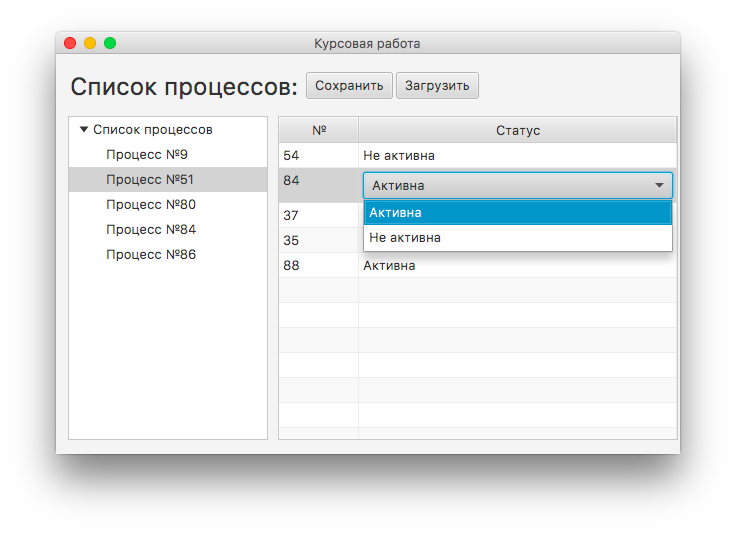
\includegraphics[width=1\textwidth]{screenshots/1.png}
    \caption{Окно программы}
    \label{fig:mesh1}
\end{figure}

Графичиский интерфейс приложения реализован при помощи технологии JavaFX и описан в файле project.fxml.
 
При запуске приложения открывается окно, которое показано на рисунке 4. Окно содержит следующие элементы: список процессов, таблица объектов памяти выбранного процесса, кнопка сохранить и кнопка загрузить. 

Список процессов реализован при помощи компонента TreeView. При инициализации приложения происходит первоначальная настройка компонента списка процессов. Первым делом устанавливается корневой элемент с надписью «Список процесов», добавляется обработчик для события клика по элементу списка процессов, который отобразит очередь объектов памяти выбранного процесса, а так же задает фабрику обработчика элементов списка процессов. Этот обработчик управляет отображением контекстного меню процесса и управляет обработкой действий для выбранного элемента конекстного меню.

Таблица объектов памяти рализована при помощи компонента TableView. При инициализации приложения происходит настройка таблицы объектов памяти. Устанавливаются маппинг номера объекта памяти соответствующей колонке в таблице объектов памяти и настройка отображения статуса объекта памяти. Отображение статуса происходит при помощи класса MemoryStatus, который определяет маппинг внутреннего значения статуса объекта памяти человеческому значению, а так же определяет, какие значения статусов возможны для установки.

Кнопки сохранения и загрузки списка процессов реализованы при помощи компонентов Button.

Обработчиком события клика по компоненту кнопки сохранения списка процессов является метод saveProcessesList контроллера MaiinController. При вызове этого метода происходит отображение диалога сохранения файла и после задания нужных параметров происходит инициализация объекта класса VirtualMachine, с помощью которого происходит сериализация списка процессов в XML файл.

Обработчиком события клика по компоненту кнопки загрузки списка процессов является метод loadProcessesList контроллера MainController. При вызове этого метода происходит отображение диалога выбра файла и после задания нужных параметров происходит инициализация объекта класса VirtualMachine, с помощью которого происходит десериализация списка процессов из выбранного XML файла с последующим отображением загруженного списка процессов в интерфейсе программы.
 
Для добавления процесса необходимо нажать правой кнопкой мыши на элемент «Список процессов» в области списка процессов. После этого отобразится контекстное меню. Это контекстное меню содержит меню «Добавить процесс», при выборе которого добавится новый процесс в объект класса ProcessList, значение которого отображено в списке процессов. 

Для добавления новой страницы памяти, удаления процесса или памяти, необходимо выбрать нужный процесс в списке процессов и нажать на него правой кнопкой мыши. После этого отобразиться контекстное меню процесса, которое содержит следующие пункты меню.

Добавить страницу памяти - при выборе этого элемента меню, будет добавлен новый объект памяти MemoryPage в выбранный процесс.

Удалить процесс - при выборе этого элемента меню, будет удален выбранный процесс из списка процессов и список процессов будет перерисован.

Удалить память - при выборе этого элемента меню, будет объект памяти будет извлечен из очереди памяти процесса.

Для изменения статуса памяти нужно выбрать необходимый процесс, после чего в таблице объектов памяти процесса нужно дважды кликнуть по статусу нужной памяти. После этого в открывшемся списке возможных статусов можно выбрать необходимый статус.

\newpage
\parindent=15mm
\section{Описание структуры проекта}

При выполнении данной работы я воспользовался строго типизированным объектно-ориентированным языком программирования Java 8, поскольку инфраструктура языка позволяет писать кроссплатформенные приложения с наименьшими трудозатратами. Для построения графического интерфейса пользователя я выбрал технологию JavaFX 8, для юнит тестирования во время разработки используется фреймворк JUnit, для сериализации используется библиотека XStream, для сборки проекта используется Maven и в качестве IDE я использовал IntelliJ IDEA CE.

Проект имеет структуру типичного Java приложения: в папке src/main находится папка основного пакета приложения, а так же папка resources, в которой находится файл project.fxml, описывающий графический интерфейс. В папке src/test находятся юнит тесты приложения, в корне проекта лежит файл pom.xml, описывающий конфигурацию Maven.

\newpage
\begin{thebibliography}{99}
\bibitem{01}	Харольд Абельсон, Джеральд Джей Сассман «Структура и Интерпретация Компьютерных Программ». Москва «Добросвет» 2010 г.
\bibitem{01}	Эрих Гамма, Ричард Хелм, Ральф Джонсон, Джон Влиссидес «Приемы объектно-ориентированного проектирования. Паттерны проектирования». Санкт-Петербург «Питер» 2016 г.
\bibitem{01}	Томас Х. Кормен, Чарльз И. Лейзерсон, Рональд Л. Ривест, Клиффорд Штайн «Алгоритмы. Построение и анализ». Москва «Вильямс» 2016 г.
\bibitem{01}	Стив Макконнелл «Совершенный код». Санкт-Петербург «BHV» 2017 г.
\bibitem{01}	Роберт К. Мартин «Чистый код: создание, анализ и рефакторинг». Санкт-Петербург «Питер» 2016 г.
\bibitem{01}	Мартин Фаулер, Дейвид Райс, Мэттью Фоммел, Эдвард Хайет, Роберт Ми, Рэнди Стаффорд «Шаблоны корпоративных приложений». Москва «Вильямс» 2016 г.
\bibitem{01}	Эрик Эванс «Предметно-ориентированное проектирование (DDD). Структуризация сложных программных систем». Москва «Вильямс» 2017 г.
\bibitem{01}	Robert Liguori, Patricia Liguori «Java Pocket Guide». Newton «O'Reilly Media» 2008 г.
\bibitem{01}	Sandi Metz, Katrina Owen «99 Bottles of OOP». 2017 г.
\bibitem{01} Kishori Sharan «Learn JavaFX 8: Building User Experience and Interfaces with Java 8». New York Apress 2015 г.
\end{thebibliography}

\newpage
\parindent=15mm
\linespread{1,5}
\section*{Полный листинг программы с краткими комментариями}
\addcontentsline{toc}{section}{Полный листинг программы с краткими комментариями}%

\renewcommand{\lstlistingname}{Листинг}
\setcounter{lstlisting}{0}

\lstinputlisting[caption=Main, style=java,  inputencoding=cp1251]{src/main/java/com/github/llxff/Main.java}

\lstinputlisting[caption=MainController, style=java,  inputencoding=cp1251]{src/main/java/com/github/llxff/MainController.java}

\lstinputlisting[caption=MemoryStatus, style=java,  inputencoding=cp1251]{src/main/java/com/github/llxff/MemoryStatus.java}

\lstinputlisting[caption=ProcessTreeCell, style=java,  inputencoding=cp1251]{src/main/java/com/github/llxff/ProcessTreeCell.java}

\lstinputlisting[caption=MemoryPage, style=java,  inputencoding=cp1251]{src/main/java/com/github/llxff/domain/MemoryPage.java}

\lstinputlisting[caption=MemoryPagesQueue, style=java,  inputencoding=cp1251]{src/main/java/com/github/llxff/domain/MemoryPagesQueue.java}

\lstinputlisting[caption=Process, style=java,  inputencoding=cp1251]{src/main/java/com/github/llxff/domain/Process.java}

\lstinputlisting[caption=ProcessesList, style=java,  inputencoding=cp1251]{src/main/java/com/github/llxff/domain/ProcessesList.java}

\lstinputlisting[caption=VirtualMachine, style=java,  inputencoding=cp1251]{src/main/java/com/github/llxff/domain/VirtualMachine.java}

\lstinputlisting[caption=project.fxml, inputencoding=utf8, style=xml]{src/main/resources/fxml/project.fxml}

\end{document}
